\ofsection{O Jogo}
%
\ofquote{"Você quer paz, melhor pegar o próximo trem."\\}{Lightning}\\\\
%
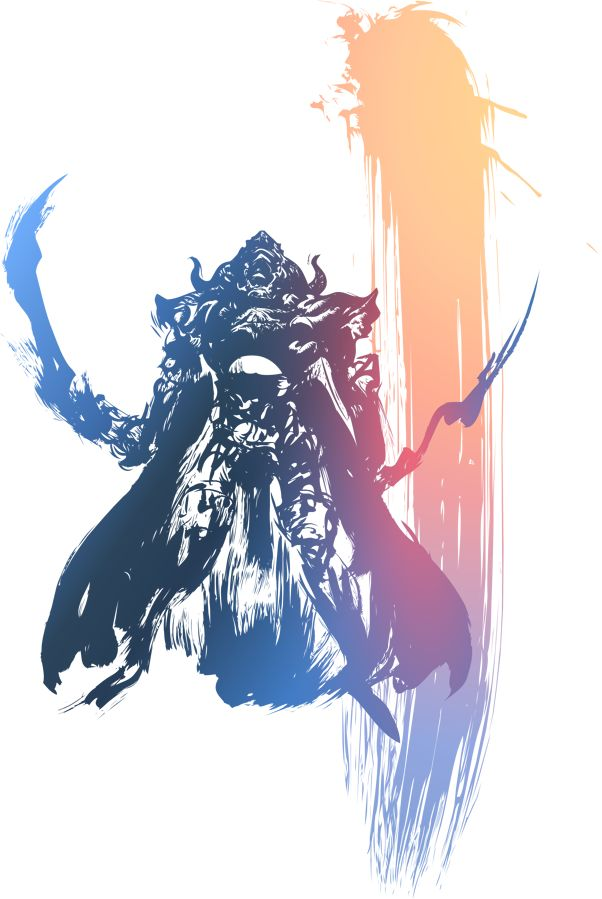
\includegraphics[width=\columnwidth]{./art/images/ff12.jpg} \\\\
%
\accf{Final Fantasy} é uma série de vídeo games em que cada título apresenta sua história, mundo e personagens únicos.
Mesmo fazendo parte da mesma série, não somente devido aos elementos recorrentes, mas também, porque suas histórias focam em um grupo de heróis que encaram um grande conflito.
Omega Fantasy é um jogo que te ajuda a criar aventuras de Final Fantasy com seus amigos e este lançamento, chamado \accf{Omega~Fantasy~II}, é uma versão melhorada da anterior. 
Para jogar, você só precisa de dados, caneta, este livro e pelo menos um amigo, embora um grupo de 4 a 6 pessoas seja o recomendado. Para completar uma aventura, seu grupo precisa se encontrar uma ou mais vezes e jogar o jogo, cada encontro é chamado de uma \accf{Sessão}.
O que não precisa ser necessariamente em pessoa, o jogo também pode ser jogado através de videoconferência.
%
\ofpar
%
Escolha uma pessoa para ser o \accf{Mestre de Jogo}~(\accf{MJ}), ele cria o mundo de jogo e narra a aventura usando o conteúdo e este livro como guia. 
Durante o jogo, ele descreve o ambiente e como ele reage às ações dos jogadores.
O MJ também representa todos os personagens não-jogadores durante interações e combates.
Todos os outros são \accf{Jogadores}, que criam e jogam o jogo da perspectiva de um \accf{Personagem} no mundo. 
Esses são os protagonistas da historia, que viajam juntos como um  \accf{Grupo} a fim de explorar o mundo, interagir com pessoas e lutar contra inimigos. 
Este livro é dividido em três sessões principais: a primeira sessão explica as regras básicas e elementos do jogo. 
A segunda, detalha as regras para a criação e desenvolvimento dos personagens dos jogadores. 
A final, foca no MJ e oferece uma variedade de guias e conteúdo para a criação do mundo de jogo.
%
\vfill
%
\ofboxwithtitle{Exemplo: Interpretação\vspace*{0.15cm}}
{
	\newcommand{\nl}{\vspace{0.2cm}\\}
	\acc{Hironobu (Mestre de Jogo):} Vocês entram nas Planícies Tempestuosas, uma vasta área desolada, coberta por uma espessa névoa e nuvens escuras. Os habitantes ergueram torres como para-raios, mas vocês podem ver que os raios atingem o chão em campo aberto.\nl
	\acc{Yoshinori (jogando como Wakka):} Nós precisamos ir para o norte, nem tão perto, nem tão longe das torres, né?\nl
	\acc{Nobuo (jogando como Rikku):} Eu quero ir para casa! Odeio raios! Odeio relâmpagos!\nl
	\acc{Tetsuya (jogando como Auron):} Essa tempestade nunca acaba. Melhor atravessar rápido.\nl
	\acc{Hironobu (Mestre de Jogo):} Vocês também podem ver uma pequena construção próxima, parece uma pousada.\nl
	\acc{Nobuo (jogando como Rikku):} Vamos dormir lá! Por favor? Sou muito jovem para morrer!\nl
	\acc{Tetsuya (jogando como Auron):} Tudo bem, vamos. Ela é pior do que a tempestade.
}
%
\vfill
%
	Rolagens de dados são usadas para decidir o resultado de ações incertas, mas a exata natureza delas depende do contexto. 
	Este jogo somente usa dados de seis lados e usa \accf{d} para se referir a eles. 
	Além do mais, usa-se, por exemplo, 4d para descrever uma rolagem de 4 dados, em que o resultado é a soma de todos eles.
	O \accf{Teste} é a principal ferramenta para ajudar o MJ a decidir e narrar o resultado das ações. 
	O MJ tanto pode pedir aos jogadores por testes ou os realizar ele mesmo, em segredo. 
	Testes geralmente são rolagens de \accf{2d} e quanto maior o resultado melhor. O resultado mínimo para ser bem sucedido é chamado de Dificuldade (\accf{DF}) e geralmente é determinado pelo MJ. 
	A DF deve ser baseada na dificuldade das ações e da proficiência do agente. A maioria das DFs variam entre 5 e 9, aquelas abaixo dessa escala são consideradas fáceis, enquanto aquelas acima, muito desafiadoras.
%
\ofpar
%
	Uma vez que 2d são rolados, o menor e o maior resultados possíveis são 2 e 12, respectivamente, que podem ser tratados como inesperadamente bons ou ruins, mas ainda assim, resultados plausíveis.
	Um teste também pode ter \accf{Vantagem} ou \accf{Desvantagem} quando as circunstâncias tem um efeito significativo sobre a ação em questão. 
	Em ambos os casos, o teste é realizado com 3d e caso seja Vantagem, somente os dois maiores serão contados e o inverso para Desvantagem. 
	Vantagem e Desvantagem cancelam a si mesmos e não acumulam.
%
\clearpage
%
\ofboxwithtitle{Exemplo: Vantagem \& Desvantagem}
{
	Cloud encontra Don Corneo em sua mansão, usando um vestido e maquiagem para o convencer de que ele é uma mulher. 
	O MJ decide que isso é uma tarefa muito difícil (DF 10), pois Cloud não se esforçou tanto assim. 
	Mas, uma vez que a sala não é bem iluminada e Don já bebeu um pouco, ele decide que o teste terá Vantagem. 
	Cloud rola 3d e obtém [6,2,6] e como somente os dois maiores dados contam, ele conseguiu o melhor resultado possível! 
	O MJ decide que Don Corneo não somente está convencido de que Cloud é uma mulher, mas também o acha tão irresistível que o leva para seu quarto para um tempo a sós.
}
%
\ofpar
%
	Outra maneira de modificar os testes é através do uso do \accf{Dado de Fortuna}. 
	No começo de cada sessão cada jogador rola 1d e o resultado é anotado, gerando a reserva (Qtd.) de Dado de Fortuna para a sessão. 
	Ao longo dela, após o jogador rolar os dados, é possível decidir remover um dos resultados da reserva e usá-lo para substituir um dado no resultado da rolagem. 
	No entanto, ao MJ também é permitido o uso de Dados de Fortuna para modificar o resultado das rolagens dos jogadores da mesma maneira. 
	Isso permite aos jogadores se beneficiar de golpes de sorte ocasionais ou motivá-los enquanto o MJ pode criar momentos de azar ou complicações. 
	Em ambos os casos, a pessoa que usa o Dado de Fortuna deve tentar dar uma justificação narrativa. Dados de Fortuna não podem ser usados enquanto em combate e qualquer dado que não seja usado é descartado ao final de cada sessão.
%
\ofpar
%
\ofboxwithtitle{Exemplo: Dado de Fortuna}
{
	Luneth explora a antiga Caverna do Altar. 
	Assim que caminha em direção a um buraco no chão, o MJ pede por um teste de DF 5, para decidir se ele o percebe ou não. Luneth obtém [3,4], o suficiente para um sucesso. 
	No entanto, o MJ decide usar um Dado de Fortuna na sua rolagem, a reserva atual de Dados de Fortuna inclui [1,3,3,5]. 
	Ele remove 1 da sua reserva e o troca pelo 4 da rolagem de Luneth. 
	Portanto, a rolagem agora é [3,1] o que significa uma falha e a reserva restante é [3,3,5]. 
	O MJ descreve o efeito da seguinte forma: à medida que Luneth tenta pisar com cuidado ao redor do buraco, ele pisa numa pedra escorregadia, tropeça e cai dentro dele. 
	Como consequência, ele se encontra em uma seção desconhecida e perigosa da caverna e tem que encontrar o caminho de volta à saída.
}
%
\ofpar
%
\ofquote{"Por que não? Nada a perder além da minha vida e isso eu ganhei de graça!"}{Setzer}\\\\
%
	 O grupo pode explorar o ambiente descrito pelo MJ à vontade. 
	 Podem procurar por coisas específicas ou apenas vagar, mas isso representa tempo. 
	 O MJ pode desenhar um mapa do local atual do grupo como um auxílio visual. 
	 Ele também é livre para impor testes em todas as ações relacionadas à exploração, como destravar uma tranca ou detectar armadilhas. 
	 O grupo pode dormir uma vez ao dia para recuperar seu PV e PM completamente, mesmo se inconsciente.
	 Para receber esse benefício, eles devem dormir em local confortável, como uma Pousada ou Tenda, por várias horas. 
	 Ao longo da aventura, o grupo interagirá com outros personagens. 
	 Estes, não-jogadores, são representados pelo MJ e agem em resposta aos jogadores.
	 Para evitar confusão, é importante deixar claro quando alguma coisa que você diz é da perspectiva de seu personagem ou sua como jogador ou MJ. 
	 Durante a interação, o MJ pode pedir testes, como para decidir se uma tentativa de convencer um personagem é bem sucedida ou não, por exemplo.
%
\vfill
%
\ofquote{"Sabe o que dizem sobre o protagonista, não? Ele nunca morre."}{Balthier}\\\\
%
Personagens se tornam mais fortes ao ganhar experiência e isso se expressa na quantidade acumulada, refletindo-se em \accf{Níveis}.
Aventureiros inexperientes começam no Nível 1 e podem progredir até, no máximo, o Nível 10. Momento em que se tornam heróis renomados. 
O MJ decide quando os personagens sobem de Nível, recomenda-se que seja ao se alcançar marcos da aventura. 
Marcos são eventos de desenvolvimento de personagens importantes, vitórias contra adversários poderosos ou a resolução de um conflito principal. 
Quando embarcar em aventuras perigosas, a \accf{Morte} é sempre uma possibilidade real, especialmente como consequência de decisões imprudentes do grupo. 
A aventura acaba se todos os membros do grupo caírem inconscientes em batalha, já que isso normalmente é seguida pela morte certa. 
Personagens também podem morrer ou deixar o grupo sob circunstâncias especiais, nesses casos o MJ toma o controle deles.
%
\ofpar
%
\ofboxwithtitle{Exemplo: Experiência \& Morte}
{
	Kain trai o grupo e se junta aos inimigos. 
	Ele luta e derrota o resto do grupo em combate, mas escolhe os deixar vivos. 
	O MJ então toma o controle dele, transformando-o em um Antagonista. 
	O grupo resolve parar os planos de Kain e seu antigo jogador resolve criar um novo personagem para os ajudar. 
	O MJ recompensa o grupo com um Nível a mais por atingir um ponto de virada na aventura.
}
%
\vfill
%
A maioria das aventuras cobrem múltiplas sessões e algumas vezes um jogador pode não ser capaz de comparecer a uma delas. 
Neste caso, o MJ e os jogadores concordam que o personagem deixa o grupo pela duração da sessão para uma \accf{Missão Pessoal}.
No início da próxima sessão, o personagem se reúne ao grupo e o jogador explica o que seu personagem tentou fazer durante sua ausência. 
Então, o MJ define uma DF para a Missão Pessoal e o jogador faz 3 testes. 
Se pelo menos 2 deles forem um sucesso, então a missão foi bem sucedida, do contrário, o personagem falhou. O MJ então descreve o curso da missão e suas consequências.
%
\clearpage
